\documentclass[a4paper,12pt]{article}

% Packages
\usepackage{graphicx}
\usepackage{amsmath}
\usepackage{geometry}
\usepackage{fancyhdr}
\usepackage{setspace}
\usepackage{titlesec}  % For title formatting
\usepackage{url}
\usepackage{hyperref}
\usepackage{comment}
\usepackage[most]{tcolorbox}
\usepackage{listings}   % <- needed for lstlisting
\usepackage{xcolor}     % <- for listings colors + table tweaks
\usepackage{booktabs}   % <- nicer tables
\usepackage{tabularx}   % <- timeline table

\geometry{margin=0.9in}
\setstretch{1.5}

% Header and Footer
\pagestyle{fancy}
\fancyhf{}
\fancyhead[L]{Progress Report}
\fancyhead[R]{
\includegraphics[width=0.1\textwidth]{Images/IOS_Tokyo.png} \thepage }

% Title Formatting
\titleformat{\section}{\normalfont\Large\bfseries}{\thesection}{1em}{}

% Listings style (simple + readable)
\lstset{
  basicstyle=\ttfamily\small,
  breaklines=true,
  frame=single,
  numbers=left,
  numberstyle=\tiny,
  keywordstyle=\color{blue!60!black},
  commentstyle=\color{green!40!black},
  stringstyle=\color{orange!60!black}
}

% Cover Page
\title{
    \vspace{2cm}
    
\includegraphics[width=0.55\textheight]{Images/IOS_Tokyo.png} \\
    \vspace{1cm}
    \textbf{\Huge NakamuLab Progress Report} \\
    \vspace{1cm}
    \large Jan 2026 -- Feb 2026 \\
    \vspace{0.5cm}

    
\includegraphics[width=0.2\textwidth]{Images/NakamuLab_logo_txt.png}
}
\author{Armando Benavidez Jr.}
\date{}

\begin{document}

% Title Page
\maketitle
\thispagestyle{empty}
\newpage

% Table of Contents
\setcounter{page}{1}
\tableofcontents
\newpage

% -----------------------
% Abstract
% -----------------------
\begin{abstract}
Coral reefs and coastal habitats are economically and ecologically critical, but they are also highly dynamic systems influenced by interacting factors such as tides, storms, turbidity, coastal development, and episodic events (e.g., runoff pulses and Sargassum influx). Diver-based underwater photomosaics and 3D reconstructions provide high-resolution, colony-scale observations, but reliable capture depends on strict field conditions (visibility, lighting stability, motion control, and repeatable survey geometry). These constraints make it difficult to collect mosaics frequently enough to observe short-timescale coastal drivers that can change hourly to daily.

This project frames underwater photomosaics and 3D reconstruction as a \textit{high-detail layer} that can be selectively repeated, while drone photomosaic surveys provide a \textit{mid-scale layer} that is faster to repeat across wider areas. Together, these tiers support coastal management questions by linking fine-scale reef condition and structure to broader spatial context (shoreline change, nearshore disturbance footprints, and patch-scale habitat shifts). A practical thesis goal is to define a small, repeatable monitoring unit (site / transect) and demonstrate a workflow that can integrate (1) sparse underwater high-detail reconstructions, (2) drone mosaics for area context, and (3) readily available long-term data layers that can be updated more frequently than diver surveys.
\end{abstract}

\newpage

% ==========================================================
% NEW SECTION: January--March Update
% ==========================================================
\section{(January--February Update) Consolidating outputs}

\tcbset{
  colback=gray!5,
  colframe=gray!40,
  boxrule=0.5pt,
  sharp corners,
  enhanced,
  fonttitle=\bfseries
}

\subsection{Completed}
\begin{itemize}
    \item Successfully ran the batch-processing pipeline on previously collected underwater photo sets to generate photo-mosaics.
 
    \item Analysis and thesis framing: deciding what measurable outputs from these mosaics will become the thesis results.
\end{itemize}

\begin{tcolorbox}[title=Current State of Data (What I Have Now)]
\begin{itemize}
    \item A set of completed underwater photomosaics (2D orthomosaics) produced from prior field surveys.
    \item Optional 3D outputs where reconstruction succeeded (dense cloud / mesh).
    \item A repeatable script-based workflow to regenerate these outputs when parameters are changed.
\end{itemize}
\end{tcolorbox}

\subsection{In Progress}
\begin{itemize}
    \item Reviewing the full set of mosaics to select a \textbf{high-quality subset} (best visibility, sharpness, consistent scale/coverage) that can serve as thesis ``core datasets.''
    \item Drafting the thesis structure and narrowing the main research question to something that can be completed within the program end date.
       \item Consolidated outputs into a single working library (mosaics, models, and exports) so they can be reviewed and compared consistently.
\end{itemize}


\subsection{In Summary}
This period focused on generating past field surveys into a usable set of processed models by running the automation script. 

The next phase is to shift effort from processing to thesis decisions: selecting a small set of high-quality mosaics, and writing the thesis around a realistic, repeatable multi-scale workflow that can be completed by the end of September.

\newpage


% ==========================================================
% Existing section: July--October Update (kept as-is, only minor safety additions)
% ==========================================================
\section{(July--October Update) Automatization of Photomosaics}

\tcbset{
  colback=gray!5,
  colframe=gray!40,
  boxrule=0.5pt,
  sharp corners,
  enhanced,
  fonttitle=\bfseries
}

\subsection{Completed}
\begin{itemize}
    \item Reorganized the photo library into a structured directory system to support automated batch processing in Metashape.
\end{itemize}

\begin{tcolorbox}[title=Folder Structure]
I created and maintained a consistent naming convention for all the folder hierarchy for the photomosaic datasets ensures that photo sets can be processed within a Metashape project while maintaining consistent naming conventions.
\begin{verbatim}
Ishigaki_2025/
└── DCIM/
    └── 100OMSYS/
        └── Ishi25_S010_0916_A1/
            ├── A/
            ├── B/
            ├── .../
            └── Z/
\end{verbatim}
\end{tcolorbox}

\begin{tcolorbox}[title=Automation Script: Image Discovery, colback=gray!5, colframe=gray!40, boxrule=0.5pt, sharp corners, enhanced, left=10mm, bottom=1mm]
The script below automatically scans alphabetized subfolders (\texttt{A--Z}) and gathers all valid image files for batch photomosaic processing.
\vspace{0.5em}

\begin{lstlisting}[language=Python]
from pathlib import Path

# Define project root folder
IMAGE_ROOT = (
    r"..\SURVEY_PHOTO_LIBRARY\Ishigaki_2025\DCIM\100OMSYS"
    r"\Ishi25_S010_0916_A1"
)
root = Path(IMAGE_ROOT)

# Identifying subdirectories (A, B, C, ...)
subdirs = [
    p for p in root.iterdir()
    if p.is_dir() and len(p.name) == 1 and p.name.isalpha()
]
subdirs.sort()

# Example: build an image list
valid_ext = {".jpg", ".jpeg", ".png", ".tif", ".tiff"}
image_list = []
for d in subdirs:
    image_list.extend([p for p in d.iterdir() if p.suffix.lower() in valid_ext])

print(
    f"Discovered {len(image_list)} images "
    f"from {len(subdirs)} subfolders: "
    f"{', '.join(p.name for p in subdirs)}"
)
\end{lstlisting}
\end{tcolorbox}

\subsection{In Progress}
\subsubsection{Automatization of Photomosaics}
\begin{figure}[h!]
    \centering
    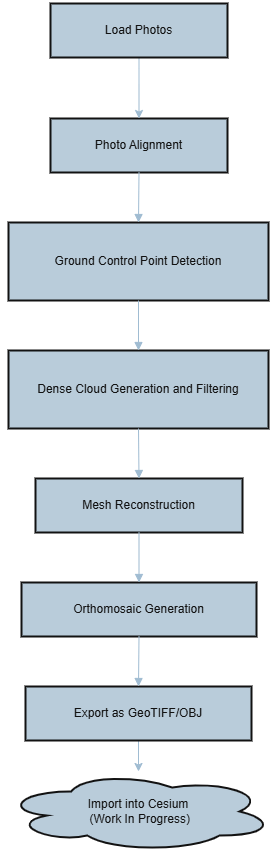
\includegraphics[width=5cm]{Images/Figures/PhotogrammetryProcessingLT.png}
    \caption{Flow chart of photomosaic data flow in Metashape}
\end{figure}

In Agisoft Metashape, the photogrammetry workflow starts by \textbf{aligning} photos to find matching points and build a sparse 3D cloud that defines how the images fit together. \textbf{Ground control points} (GCPs) are then imported (if available). From there, a \textbf{dense cloud} is generated to capture detailed surface geometry, and low-confidence points are filtered out. The next step is \textbf{mesh reconstruction}, which connects those points into a continuous 3D surface. Once the geometry is complete, Metashape projects the photos onto it to create a georeferenced orthomosaic. Finally, outputs are exported for downstream analysis and visualization.

\subsubsection{Scripting}

\tcbset{colback=gray!5,colframe=gray!40,boxrule=0.5pt,sharp corners,enhanced}

\begin{tcolorbox}[title=Add Photos]
\texttt{chunk.addPhotos(image\_list)} --- Loads all images from A..Z folders.
\end{tcolorbox}

\begin{tcolorbox}[title=Photo Alignment]
\texttt{chunk.matchPhotos(...)} then \texttt{chunk.alignCameras()} --- Finds matching features across images.
\end{tcolorbox}

\begin{tcolorbox}[title=GCP Import \& Optimization (optional)]
\texttt{chunk.importReference(...)} and \texttt{chunk.optimizeCameras(...)} --- Brings in control points and refines alignment for scaling/georeferencing.
\end{tcolorbox}

\begin{tcolorbox}[title=Dense Cloud Generation \& Filtering]
\texttt{chunk.buildDepthMaps(...)} --- Computes depth for each image to create dense geometry.
\end{tcolorbox}

\begin{tcolorbox}[title=Mesh Reconstruction]
\texttt{chunk.buildModel(...)} --- Converts depth information into a continuous 3D surface (mesh).
\end{tcolorbox}

\begin{tcolorbox}[title=Orthomosaic Generation]
\texttt{chunk.buildOrthomosaic(...)} --- Projects the photos onto the mesh and blends mosaic image.
\end{tcolorbox}

\begin{tcolorbox}[title=Export as GeoTIFF/OBJ]
\texttt{chunk.exportOrthomosaic(...)} --- Writes the orthomosaic to disk.
\end{tcolorbox}

The following is a link to the Metashape Python API:
\href{https://www.agisoft.com/pdf/metashape_python_api_2_2_0.pdf}{link}.

\subsection{In Summary}
I’m organizing my underwater photos to track completed locations and outline the photomosaic workflow. Using the Metashape GUI for each dataset can be slow and repetitive. Agisoft Metashape offers a Python API that I can integrate into my project pipeline, which supports automation of photomosaic creation and reduces manual work through the GUI.

\end{document}